\documentclass{article}

\usepackage[italian]{babel}     %testi autogenerati italiano
\usepackage{minted}             %per codice vhdl bello
\usepackage{tikz}               %per disegno fsm
\usetikzlibrary{automata, positioning, arrows}
\usepackage{circuitikz}         %per disegno componente
\usepackage{graphicx}           %per importare immagini
\usepackage{geometry}           %per gestire margini e spostamenti
\geometry {
    top=20mm,
    bmargin=20mm,
}
\usepackage{array}              %per colonne di width fissata
\usepackage{subcaption}         %tabelle divise
\usepackage{hyperref}           %links
\hypersetup{
    colorlinks=true,
    linkcolor=black,
    urlcolor=blue
}
%\usepackage[bottom]{footmisc}   %footnotes fissate a piè pagina
\usepackage{booktabs}           %per tabitem in tabular
\newcommand{\tabitem}{~~\llap{\textbullet}~~}
\renewcommand*{\thefootnote}{[\arabic{footnote}]}

\begin{document}

\setlength\parindent{0pt} %noindent automatico
\setlength\parskip{1em}

\begin{titlepage}
    \centering
    \hrule

    \vspace{0,5cm}
    {
        \normalsize Politecnico di Milano\\
        Dipartimento di Elettronica, Informazione e Bioingegneria
    }

    \vspace{5cm}
    {\Huge \textbf{Progetto di Reti Logiche\\
            A.A. 2021/2022}\\}

    \vspace{0,5cm}
    \large {Prof. Palermo Gianluca}

    \vspace{5cm}
    {
        \large
        \begin{tabular}{c c}
            Dario Simoni \\
            (Codice Persona: 10697990, Matricola: 932957) \\
        \end{tabular}

    }

    \vspace{6.5cm}


    \hrule

\end{titlepage}

\pagebreak

\tableofcontents

\pagebreak

\section{Requisiti di progetto} %1
\subsection{Descrizione del problema} %1.1
Si vuole realizzare un modulo HW (descritto in VHDL) che si interfacci con una memoria e che
ricevendo in ingresso un flusso continuo X da 1 bit restituisca un nuovo flusso continuo Y da 1 bit.
\par
Il flusso continuo X è generato da una seguenza continua di parole serializzate in base alla specifica, mentre il flusso continuo Y restituisce il doppio dei bit rispetto al flusso X.
\vspace{0,2cm} %un po' di spazio

\subsection{Interfaccia del componente} %1.2
Il componente da descrivere deve avere la seguente interfaccia

\begin{minted}{vhdl}
    entity project_reti_logiche is
	  port (
	    i_clk     : in  std_logic;
	    i_rst     : in  std_logic; 
	    i_start   : in  std_logic; 
	    i_data    : in  std_logic_vector (7 downto 0);
	    o_address : out std_logic_vector (15 downto 0);
    	o_done    : out std_logic; 
    	o_en      : out std_logic;
	    o_we      : out std_logic;
	    o_data    : out std_logic_vector (7 downto 0) 
	  );
    end project_reti_logiche;
\end{minted}
\vspace{0,2cm} %un po' di spazio

In particolare:
\begin{itemize}
    \item   il nome del modulo deve essere project\_reti\_logiche;
    \item   \texttt{i\_clk} è il segnale di CLOCK in ingresso generato dal TestBench;
    \item   \texttt{i\_rst} è il segnale di RESET che inizializza la macchina pronta per ricevere il primo segnale di START;
    \item   \texttt{i\_start} è il segnale di START generato dal Test Bench;
    \item   \texttt{i\_data} è il segnale (vettore) che arriva dalla memoria in seguito a una richiesta di lettura;
    \item   \texttt{o\_address} è il segnale (vettore) di uscita che manda l’indirizzo alla memoria;
    \item   \texttt{o\_done} è il segnale di uscita che comunica la fine dell’elaborazione e il dato di uscita scritto in memoria;
    \item   \texttt{o\_en} è il segnale di ENABLE da mandare alla memoria per poter comunicare (sia in lettura che in scrittura);
    \item   \texttt{o\_we} è il segnale di WRITE ENABLE da mandare alla memoria (\texttt{=1}) per poter scriverci. Per leggere da memoria esso deve essere \texttt{0};
    \item   \texttt{o\_data} è il segnale (vettore) di uscita dal componente verso la memoria.
\end{itemize}

\pagebreak

\vspace{0,2cm}

\subsection{Descrizione della memoria e dell'interazione con il componente} %1.3
Il modulo riceve in ingresso una sequenza continua di W parole, ognuna di 8 bit, e
restituisce in uscita una sequenza continua di Z parole, ognuna da 8 bit. Ognuna delle
parole di ingresso viene serializzata; in questo modo viene generato un flusso continuo U da
1 bit. Su questo flusso viene applicato il codice convoluzionale ½ (ogni bit viene codificato
con 2 bit); questa operazione genera in uscita un
flusso continuo Y. Il flusso Y è ottenuto come concatenamento alternato dei due bit di uscita.
Utilizzando la notazione riportata in figura, il bit uk genera i bit p1k e p2k che sono poi
concatenati per generare un flusso continuo yk (flusso da 1 bit). La sequenza d’uscita Z è la
parallelizzazione, su 8 bit, del flusso continuo yk
\vspace{0,3cm}

\begin{center}
    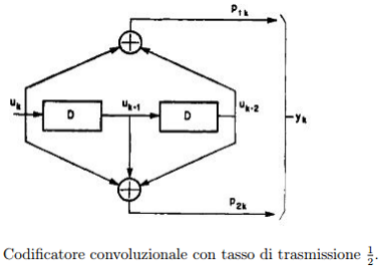
\includegraphics[scale=1]{./photo1.png}}
\end{center}

\vspace{0,2cm}

\begin{center}
	\begin{tabular}{ |c|c|c| }
		\hline
		Indirizzo RAM & Contenuto & Azione \\ 
		\hline
		0 & byte - lunghezza sequenza di ingresso & lettura \\
		\hline
		1 & byte - prima parola da codificare & lettura \\
		\hline
		2 & byte - seconda parola da codificare & lettura \\
		\hline
		\vdots & indirizzi potenzialmente non utili & \vdots \\
		\hline
		1000 & byte - prima parola in uscita & scrittura \\
		\hline
		1001 & byte - seconda parola in uscita & scrittura \\
		\hline
		1002 & byte - terza parola in uscita & scrittura \\
		\hline
		1003 & byte - quarta parola in uscita & scrittura \\
		\hline
		\vdots & indirizzi potenzialmente non utili & \vdots \\
		\hline
	\end{tabular}
	\captionof{table}{Rappresentazione della RAM} 
\end{center}

\vspace{0,5cm}

La lunghezza del flusso U è 8*W, mentre la lunghezza del flusso Y è 8*W*2 (Z=2*W).
Il convolutore è una macchina sequenziale sincrona con un clock globale e un segnale di
reset con il seguente diagramma degli stati che ha nel suo 00 lo stato iniziale, con uscite in
ordine P1K, P2K (ogni transizione è annotata come Uk/p1k, p2k).

\pagebreak

\begin{center}
    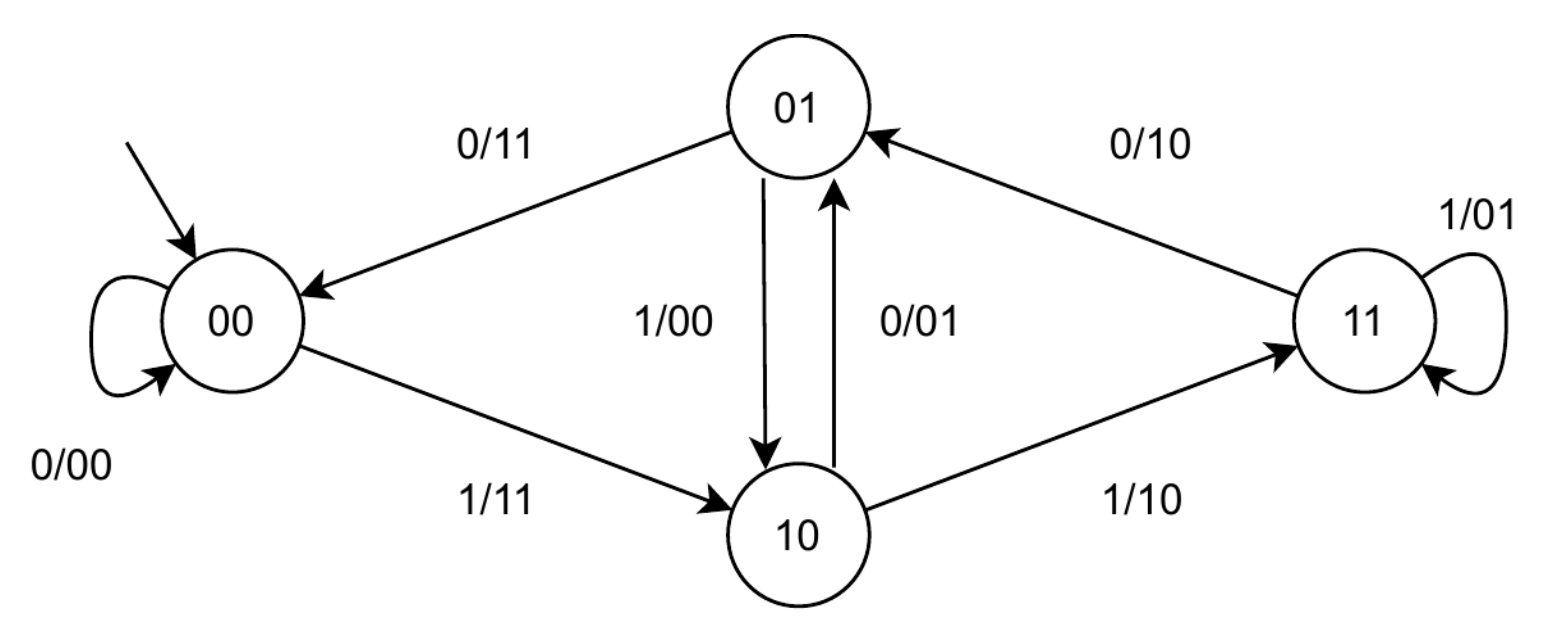
\includegraphics[scale=0.3]{./photo2.png}}
\end{center}

\subsection{Esempio di funzionamento} %1.4
\label{sec:esempio}
%Si riporta in seguito un esempio di elaborazione compiuta su un'immagine di test:

\begin{center}
    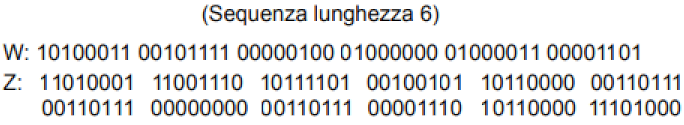
\includegraphics[scale=0.65]{./photo3.png}}
\end{center}
\begin{center}
    W \texttt{=} Input \texttt{|} Z \texttt{=} Output
\end{center}
\vspace{0,2cm}
\begin{table}[h]
    \centering
    \label{tab:esMEM}
    \begin{tabular}{c|c}
        addr. & data \\
        \hline \hline
        0     & 6    \\
        1     & 163  \\
        2     & 47   \\
        3     & 4    \\
        4     & 64   \\
        5     & 67   \\
        6     & 13   \\
        \texttt{[...]} &      \\ 
        1000  & 209  \\
        1001  & 206  \\
        1002  & 189  \\
        1003  & 37   \\
        1004  & 176  \\
        1005  & 55   \\
        1006  & 55   \\
        1007  & 0    \\
        1008  & 55   \\
        1009  & 14   \\
        1010  & 176  \\
        1011  & 232  \\
    \end{tabular}\hspace{15pt}
\end{table}

\pagebreak

\section{Architettura del componente} %2
Ho scelto di descrivere un modulo hardware tramite architettura \emph{behavioral} (comportamentale) in linguaggio VHDL, esso opera su una macchina a stati finiti che realizza l'argoritmo esposto più avanti.
\vspace{0,2cm}
\subsection{Descrizione ad alto livello}
L'algoritmo definito allo svolgimento dell’operazione può essere schematizzato secondo i seguenti passaggi chiave:
\begin{itemize}
    \item   [1)]    Lettura del numero di parole \texttt{to\_be\_processed};
    \item   [2)]    Ciclo per leggere i bit della parola in ingresso ed elaborarli nella FSM;
    \item   [3)]    Scrittura della prima parola in uscita;
    \item   [4)]    Scrittura della seconda parola in uscita;
    \item   [5)]    Aumento del contatore \texttt{words\_processed};
    \item   [6)]    Ripeto dal punto \texttt{2)} fino a quando \texttt{words\_processed=to\_be\_processed} e poi procedo al DONE.
\end{itemize}

\subsection{Macchina a stati finiti} %2.1
L’FSM schematizzata è composta da 10 stati, suddivisibili in 3 gruppi principali descritti più avanti.

\subsubsection{Stati ausiliari} %2.1.1
Gruppo di stati che realizza: inizio e fine del processo, richiesta di lettura e attesa della memoria.
\begin{itemize}
    \item [i.]     \textbf{\texttt{START} - wait start}: stato di attesa del segnale di \texttt{i\_start}. \\
          In qualsiasi momento dell’elaborazione, se il segnale \texttt{i\_rst} è rilevato alto\footnotemark, anche non in corrispondenza di \texttt{i\_clk}, la macchina viene riportata in questo stato, tornando in attesa di un nuovo segnale di inizio elaborazione.\par
          Al verificarsi della condizione \texttt{i\_start = 1} vengono inizializzati tutti i valori necessari al processo, prima di passare allo stato successivo;
          \footnotetext{Si è supposto che il segnale \texttt{i\_start} vada a 0 per il periodo in cui \texttt{i\_rst} è 1 in caso di reset.}
    \item [ii.]    \textbf{\texttt{WAIT\_START} - wait memory}: stato in cui porto \texttt{o\_en} a 1 ed \texttt{o\_address} all’indirizzo della RAM che deve essere letto;
    \item [iii.]    \textbf{\texttt{WAIT\_READ\_NUMBER\_OF\_WORD} - wait memory}: stato di attesa in cui permetto a \texttt{to\_be\_processed} di valere l'intero assegnatogli;
    \item [iv.]     \textbf{\texttt{PREPARE\_BIT\_READ} - read request}: stato in cui porto \texttt{o\_we} a 0 e \texttt{o\_address} all’indirizzo della RAM che deve essere letto;
    \item [v.]     \textbf{\texttt{WAIT\_PREPARE\_BIT\_READ} - wait memory}: stato di attesa in cui permetto a \texttt{PREPARE\_BIT\_READ} di aggiornare i valori;
    \item [vi.]    \textbf{\texttt{WAIT\_READ\_BIT} - wait memory}: stato di attesa in cui permetto a \texttt{READ\_BIT} di aggiornare i valori;
    \item [vii.]    \textbf{\texttt{WAIT\_WRITE\_WORD\_ONE} - wait memory}: stato di attesa in cui permetto a \texttt{PREPARE\_BIT\_READ} di aggiornare i valori;
    \item [viii.]    \textbf{\texttt{WAIT\_WRITE\_WORD\_TWO} - wait memory}: stato di attesa in cui permetto a \texttt{PREPARE\_BIT\_READ} di aggiornare i valori;
    \item [ix.]      \textbf{\texttt{DONE} - done}: stato in cui \texttt{o\_done} viene posto a \texttt{‘1’} per segnalare la fine dell’elaborazione. A questo punto, si attende un valore di \texttt{i\_start} basso per tornare in \texttt{START} e poter ricevere nuove parole;
\end{itemize}


\subsubsection{Lettura della memoria} %2.1.2
Gruppo di stati che si occupa della lettura delle informazioni e della loro elaborazione in \texttt{word1} e \texttt{word2}.
\begin{itemize}
    \item [x.]     \textbf{\texttt{READ\_NUMBER\_OF\_WORD} - read \texttt{to\_be\_processed}}: stato in cui viene popolato il valore \texttt{to\_be\_processed} con il numero di parole da processare;
    \item [xi.]    \textbf{\texttt{READ\_BIT} - read bit}: stato in cui percorrendo la FSM leggo un bit, lo processo ottenendone due e proseguo di posizione.
    Questo stato si occupa anche del controllo \texttt{to\_be\_processed=words\_processed} che porta allo stato di DONE;
\end{itemize}

\subsubsection{Scrittura delle parole nella memoria} %2.1.3
Gruppo di stati che si occupa della scrittura nella memoria delle parole ottenute.\par
\begin{itemize}
    \item [xii.]   \textbf{\texttt{WRITE\_WORD\_ONE} - write data}: stato in cui metto il valore dell'\texttt{std\_logic\_vector} word1 nella memoria;
    \item [xiii.]   \textbf{\texttt{WRITE\_WORD\_TWO} - write data}: stato in cui metto il valore dell'\texttt{std\_logic\_vector} word2 nella memoria;
\end{itemize}

\clearpage

\subsubsection{Diagramma della macchina a stati finiti}
%immagine FSM
\begin{figure}[ht]
    \centering
    \begin{tikzpicture}[->,>=stealth',shorten >=1pt,auto,node distance=3cm, semithick, initial text=$ $, initial where= above]
        \node[state, initial]           (0) {\texttt{START}};
        \node[state, right of=0]        (1) {\texttt{WAIT}};
        \node[state, right of=1]        (2) {\texttt{READ\_0}};
        \node[state, right of=2]        (3) {\texttt{WAIT}};
        \node[state, below=4.5cm of 3]        (4) {\texttt{PREPARE}};
        \node[state, left of=4]         (5) {\texttt{WAIT}};
        \node[state, left of=5]         (6) {\texttt{READ\_BIT}};
        \node[state, below of=6]        (7) {\texttt{WAIT}};
        \node[state, left of=6]         (8) {\texttt{WRITE\_1}};
        \node[state, above of=8]        (9) {\texttt{WAIT}};
        \node[state, right of=9]        (10) {\texttt{WRITE\_2}};
        \node[state, right of=10]       (11) {\texttt{WAIT}};
        \node[state, below of=8]        (12) {\texttt{DONE}};

        \draw
        (0)  edge[loop left]      node {\texttt{i\_start=0}}             (0)
        (0)  edge                 node {\texttt{i\_start=1}}             (1)
        (1)  edge                 node {\texttt{}}                       (2)
        (2)  edge                 node {\texttt{}}                       (3)
        (3)  edge                 node {\texttt{}}                       (4)
        (4)  edge                 node {\texttt{}}                       (5)
        (5)  edge                 node {\texttt{}}                       (6)
        (6)  edge                 node {\texttt{\emph{cond3}}}           (7)
        (7)  edge                 node {\texttt{}}                       (6)
        (6)  edge                 node {\texttt{\emph{cond2}}}           (8)
        (8)  edge                 node {\texttt{}}                       (9)
        (9)  edge                 node {\texttt{}}                       (10)
        (10) edge                 node {\texttt{}}                       (11)
        (11) edge                 node {\texttt{}}                       (4)
        (6)  edge                 node {\texttt{\emph{cond1}}}           (12)
        (12) edge[loop left]      node {\texttt{i\_start=1}}             (12)
        (12) edge[bend left]      node {\texttt{i\_start=0}}             (0)
    \end{tikzpicture}
    \label{fig:fsm}
\end{figure}
\vspace{0,2cm}

In figura sono state utilizzate le seguenti abbreviazioni:
\vspace{-.1cm}
    \def\arraystretch{1.2} %un po' di padding
    \begin{tabular}{||c|c||}
        \hline
        \texttt{\emph{cond1}} & \texttt{to\_be\_processed = words\_processed}                  \\\hline
        \texttt{\emph{cond2}} & \texttt{!cond1 \& count = 8}                                             \\\hline
        \texttt{\emph{cond3}} & \texttt{!cond1 \& count != 8}                                             \\\hline
    \end{tabular}
\vspace{0,2cm}

Per ogni stato dell'FSM è presente un arco uscente implicito diretto verso lo stato di reset, che permette di interrompere in qualsiasi momento l'operazione corrente, tramite un segnale \texttt{i\_rst=1}.
\vspace{0,2cm}

\subsection{Scelte progettuali e ottimizzazioni} %2.3
Ho scelto di progettare un componente sensibile al clock su \emph{rising\_edge}.\par
Nell’implementazione dell’algoritmo vorrei far notare la scelta di mantenere la FSM della specifica implementata tramite if/elsif con dei signal boolean che simulano il passaggio da uno stato ad un altro.

Si noti che nella mia implementazione ci vogliono due cicli di clock per la lettura di un singolo bit per parola, portando la lettura ed elaborazione di una parola a minimo 16 cicli di clock.
Nella processione della parola ricevuta mi salvo per ogni bit i due bit, ricevuti dalla FSM, nelle posizioni corrispondenti di due \texttt{std\_logic\_vector}.

Infine si noti che la lettura dei bit avviene 8 volte per leggere una parola intera prima di passare allo stato di \texttt{WRITE\_1}.

\pagebreak

Di seguito è presente il blocco if/elsif utilizzato per la processione dei bit delle parole attraverso la FSM data:
\begin{center}
    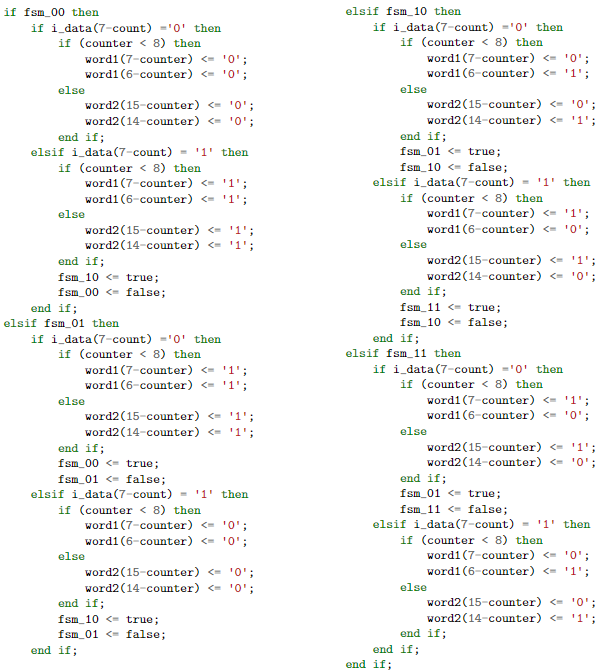
\includegraphics[scale=3]{./photo4.png}}
\end{center}

\pagebreak

\section{Risultati sperimentali} %3
\subsection{Casi di test} %3.1
Il corretto funzionamento del componente sviluppato è stato verificato tramite numerosi \emph{TestBench}.\par In particolare, ho scelto di concentrare l’attenzione su diversi casi critici possibili durante l’esecuzione e sul corretto calcolo di tutti i valori utilizzati. Di seguito una breve lista di condizioni e test più significativi:

\begin{itemize}
    \item   Corretta attenzione nei boolean della fsm \texttt{(fsm\_00 fsm\_01 fsm\_10 fsm\_11)};
    \item   Condizione particolare: \texttt{to\_be\_processed = 0};
    \item   Casi di test con numero di parole massivo;
    \item   Caso di reset dell’elaborazione;
    \item   Corretto rapporto dei segnali \texttt{i\_rst}, \texttt{i\_start} e \texttt{o\_done} durante   l’esecuzione.
\end{itemize}


È stato particolarmente utile utilizzare l'analisi grafica dei segnali di input/output del modulo.
\vspace{0,2cm}

\begin{figure}[ht]
    \centering
    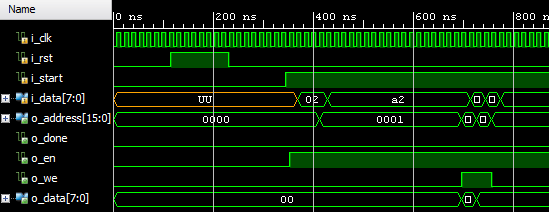
\includegraphics[scale=0.9]{./photo5.png}
    \caption{Analisi dei segnali di input e output nell'elaborazione di più parole consecutive.}
\end{figure}
\vspace{0,5cm}

Si sono utilizzati diversi \emph{TestBench} con caratteristiche differenti e dimensioni variabili fino alle \texttt{5000} parole, redatti manualmente o auto-generati tramite uno script python.
\vspace{0,2cm}

\clearpage
\pagebreak

\subsection{Risultati sperimentali}
Il report di sintesi ha evidenziato l’utilizzo nell’area del modulo sintetizzato dei seguenti componenti:

\begin{table}[ht]
    \centering
    \small
    \def\arraystretch{1.3} %un po' di padding
    \caption{Risultati della tabella\footnotemark \emph{"utilization"} generata dalla simulazione di \emph{post-synthesis}.}
    \begin{tabular}[width=4cm]{|| l | r | r ||}
        \hline
        Risorsa       & Stima & Utilizzo $\%$              \\
        \hline \hline
        \texttt{LUT}  & 397   & 0.51                       \\ \hline
        \texttt{FF}   & 163    & 0.10                       \\ \hline
        \texttt{IO}   & 38    & 15.20                      \\ \hline
        \texttt{BUFG} & 1     & 3.13                       \\ \hline
    \end{tabular}
\end{table}
\footnotetext{Percentuali riferite alla scheda \texttt{FPGA} utilizzata: \texttt{xc7z030fbv676-2}.}
\vspace{0,2cm}

\subsection{Risultati di simulazione}
Per tutti i casi di test e \emph{TestBench} utilizzati, compreso quello delle 5000 parole, sono state svolte con successo le simulazioni richieste dalle specifiche di progetto.

Inoltre la condizione del periodo di clock di "almeno 100 ns" è stata verificata con il seguente constraint:

    \texttt{create\_clock -period 100 -name clock [get\_ports i\_clk]}
\end{tabular}\vspace{0,2cm}

\section{Conclusioni}
A seguito di questo processo posso affermare di aver ampliato di sicuro le mie conoscenze sulla progettazione di un componente con le caratteristiche simili a quello proposto e ritengo che l'architettura proposta rispecchi a pieno le specifiche.

\clearpage

\end{document}
